\documentclass[11pt,letterpaper]{article}
\usepackage[utf8]{inputenc}
\usepackage[T1]{fontenc}
\usepackage{lmodern} % Classic, highly legible typeface
\usepackage{amsmath, amssymb, amsfonts}
\usepackage[margin=2.5cm]{geometry}
\usepackage{fancyhdr}
\usepackage{tabularx}
\usepackage{enumitem}
\usepackage[most]{tcolorbox}
\usepackage{colortbl}
\usepackage{xcolor}
\usepackage{tikz}
\usetikzlibrary{arrows.meta}
\renewcommand{\figurename}{Figure}

% ============ REFERENCE COLOR PALETTE ============
\definecolor{tealmain}{HTML}{007F80}    % Main teal (headings and equations)
\definecolor{darkforest}{HTML}{243F26}  % Deep forest green (subheadings and key concepts)
\definecolor{darkslate}{HTML}{172D3C}   % Dark slate blue (body text and crisp reading)
\definecolor{graysub}{HTML}{546E7A}     % Secondary blue-gray (metadata)
\definecolor{creambg}{HTML}{FFFAF0}     % Soft ivory (warm background for main boxes)
\definecolor{tealacc}{HTML}{00897B}     % Emerald green accent (properties)
\definecolor{orangeacc}{HTML}{D96B27}   % Warm orange (challenges or warnings)
\definecolor{darkbrown}{HTML}{5A3A24}   % Dark brown accent (graphics)

% ============ HEADERS / FOOTERS ============
\setlength{\headheight}{24pt}
\pagestyle{fancy}
\fancyhf{}
\fancyhead[L]{\textcolor{darkforest}{\textbf{\small Classical Mechanics}}}
\fancyhead[R]{\textcolor{tealmain}{\textbf{\small Undergraduate Notes}}}
\fancyfoot[C]{\textcolor{graysub}{\thepage}}
\renewcommand{\headrulewidth}{0.7pt}
\renewcommand{\headrule}{\hbox to\headwidth{\color{tealmain!60}\leaders\hrule height \headrulewidth\hfill}}

% Stylized square bullets
\setlist[itemize]{label={\small\textcolor{tealmain}{$\blacksquare$}}}

% ============ SECTION COMMANDS WITH COLORED RULE ============
\newcommand{\manualsection}[1]{%
  \vspace{0.35cm}
  {\Large\bfseries\color{darkslate} #1}\\[2pt]
  {\color{tealmain!70}\rule{\linewidth}{1.2pt}}\\[0.25cm]
}

\newcommand{\manualsubsection}[1]{%
  \vspace{0.2cm}\noindent{\bfseries\color{tealmain} #1}\\[0.15cm]
}

% ============ CONTENT BOXES ============
% Main box (formal definitions in teal)
\newtcolorbox{infobox}[2][tealmain]{
  enhanced, breakable,
  colback=creambg!40!white, colframe=#1!75!black,
  boxrule=0.8pt, arc=2mm,
  left=9pt, right=9pt, top=8pt, bottom=8pt,
  before upper={\textbf{\color{#1!90!black}\large #2}\\[3pt]{\color{#1!40}\rule{\linewidth}{0.6pt}}\\[6pt]}
}

% Properties / kinematics box (soft mint background)
\newtcolorbox{ejerciciobox}[1]{
  enhanced, breakable,
  colback=tealmain!5!white, colframe=tealmain!80!black,
  boxrule=0.8pt, arc=2mm,
  left=9pt, right=9pt, top=8pt, bottom=8pt,
  before upper={\textbf{\color{tealmain!95!black}\large #1}\\[3pt]{\color{tealmain!35}\rule{\linewidth}{0.6pt}}\\[6pt]}
}

% Structural concepts box (forest green / dark forest)
\newtcolorbox{teobox}[1]{
  enhanced, breakable,
  colback=darkforest!5!white, colframe=darkforest!85!black,
  boxrule=1pt, arc=2mm,
  left=9pt, right=9pt, top=8pt, bottom=8pt,
  before upper={\textbf{\color{darkforest!95!black}\large #1}\\[3pt]{\color{darkforest!35}\rule{\linewidth}{0.7pt}}\\[6pt]}
}

% Highlighting for key terms
\newcommand{\term}[1]{\textbf{\color{tealmain}#1}}
\newcommand{\termb}[1]{\textbf{\color{darkforest}#1}}


% Style aliases retained to preserve the document's commands.
\colorlet{pinkmain}{tealmain}
\colorlet{purplesec}{darkforest}
\colorlet{darktext}{darkslate}

% Challenge box retained and harmonized with the reference palette.
\newtcolorbox{retobox}[1]{
  enhanced, breakable,
  colback=orangeacc!4!white, colframe=orangeacc!75!black,
  boxrule=0.9pt, arc=2mm,
  left=9pt, right=9pt, top=8pt, bottom=8pt,
  before upper={\textbf{\color{orangeacc!90!black}\large #1}\\[3pt]{\color{orangeacc!35}\rule{\linewidth}{0.6pt}}\\[6pt]}
}

% Latin Modern typography for text, mathematics, and vector labels.
\renewcommand{\familydefault}{\rmdefault}
\tikzset{every node/.append style={font=\rmfamily}}
\usepackage{etoolbox}
\AtBeginEnvironment{equation}{\color{tealmain}}

% Integrated vector graphics, without external images or background fill.
\usepackage{pgfplots}
\usepgfplotslibrary{groupplots}
\pgfplotsset{compat=1.18}
\pgfplotsset{mecanica axis/.style={
  axis background/.style={fill=none},
  axis line style={graysub},tick style={graysub},
  tick label style={font=\rmfamily\small,text=graysub},
  label style={font=\rmfamily\small,text=darkslate},
  scaled ticks=false,
}}
\usepackage{placeins}
\begin{document}
\color{darkslate} % Reference reading color.


% ============ TITLE PAGE ============
\begin{center}
    {\LARGE \textbf{\color{pinkmain}Lagrangian Mechanics: Generalized Coordinates}}\\[0.2cm]
    {\Large \textcolor{purplesec}{\textbf{Classical Mechanics -- Undergraduate Notes}}}\\[0.4cm]
    {\large \textcolor{graysub}{Gabriel Velázquez}}\\[0.6cm]
\end{center}

\manualsection{1. Introduction and Degrees of Freedom}

In the conventional Newtonian formulation, the instantaneous spatial position of a set of $N$ point particles is parametrized using position vectors in Cartesian coordinates:
\begin{equation}
    \mathbf{r}_i = (x_i, y_i, z_i), \quad i = 1, \dots, N.
\end{equation}
To describe this unconstrained ensemble completely, $3N$ independent scalar coordinates are required. We therefore say that the system has $3N$ \term{degrees of freedom}.

\begin{infobox}[purplesec]{Definition 1.1 (Degrees of Freedom and Reduction by Constraints)}
If a physical system of $N$ particles is subject to $k$ independent holonomic constraints, each constraint reduces the number of required variables by one. Therefore, the total number of independent \termb{degrees of freedom} $s$ (which determines the dimension of configuration space) is:
\begin{equation}
    s = 3N - k.
\end{equation}
\end{infobox}

\manualsection{2. Constraints}

A \term{constraint} in classical mechanics is any geometric, kinematic, or physical limitation imposed on a system that prevents its free motion in Cartesian coordinate space.

\manualsubsection{Holonomic vs. Nonholonomic Classification}

\begin{infobox}[pinkmain]{Definition 2.1 (Holonomic Constraints)}
A constraint is \term{holonomic} when it can be formulated as a finite algebraic equation involving only particle positions and time:
\begin{equation}
    f_\alpha(\mathbf{r}_1, \mathbf{r}_2, \dots, \mathbf{r}_N, t) = 0, \quad \alpha = 1, \dots, k.
\end{equation}
\textbf{Example:} The confinement of a particle to the surface of a fixed sphere of constant radius $a$, described by $x^2 + y^2 + z^2 - a^2 = 0$.
\end{infobox}


% BEGIN ADDITIONAL_GRAPHICS: circular_constraint
\begin{figure}[!htbp]
\centering
% Exact geometry; theta=0.65 rad is measured from the downward vertical.
\begin{tikzpicture}[x=2.25cm,y=2.25cm,>=Stealth]
  \draw[->,graysub] (-1.3,0)--(1.4,0) node[right] {$x/\ell$};
  \draw[->,graysub] (0,-1.3)--(0,1.35) node[above] {$y/\ell$};
  \foreach \u in {-1,1} {
    \draw[graysub] (\u,0.035)--(\u,-0.035) node[below=3pt] {\small $\u$};
    \draw[graysub] (0.035,\u)--(-0.035,\u) node[left=3pt] {\small $\u$};
  }
  \node[below left,graysub] at (0,0) {\small $0$};
  \draw[tealacc,very thick] (0,0) circle[radius=1];
  \coordinate (P) at ({sin(deg(0.65))},{-cos(deg(0.65))});
  \draw[darkbrown,thick] (0,0)--(P) node[midway,right=4pt] {$\ell$};
  \fill[darktext] (0,0) circle[radius=1.5pt];
  \fill[darkbrown] (P) circle[radius=2.8pt];
\end{tikzpicture}
\caption{Planar example of a holonomic constraint: $x^2+y^2-\ell^2=0$, with fixed $\ell>0$. The circle shows the admissible positions, and the segment indicates the radius $\ell$. The axes are normalized by $\ell$; no time evolution is prescribed.}
\label{fig:ligadura_circular_python}
\end{figure}
\FloatBarrier

% END ADDITIONAL_GRAPHICS: circular_constraint
\begin{teobox}{Nonholonomic Constraints}
A constraint is \termb{nonholonomic} if it cannot be reduced to integrable algebraic relations among position coordinates. These include:
\begin{itemize}
    \item \textbf{Geometric inequalities:} Constraints of the form $f(\mathbf{r}_1, \dots, \mathbf{r}_N) \ge 0$ (e.g., a particle confined inside a spherical container of radius $a$, $r \le a$).
    \item \textbf{Nonintegrable differential relations:} Kinematic constraints among coordinate and time differentials:
    \begin{equation}
        \sum_{i=1}^n A_{\alpha i} \, dq_i + B_\alpha \, dt = 0,
    \end{equation}
    typical of pure rolling without slipping.
\end{itemize}
\end{teobox}

\manualsubsection{Scleronomous vs. Rheonomous Classification}

\begin{itemize}
    \item \textbf{Scleronomous Constraint:} The constraint does not depend explicitly on time:
    \begin{equation}
        f(\mathbf{r}_1, \dots, \mathbf{r}_N) = 0.
    \end{equation}
    \item \textbf{Rheonomous Constraint:} Time appears explicitly in its formulation:
    \begin{equation}
        f(\mathbf{r}_1, \dots, \mathbf{r}_N, t) = 0.
    \end{equation}
    \textit{Example:} A pendulum whose support oscillates vertically according to an imposed time law $z_0(t) = A\cos(\omega t)$.
\end{itemize}

\manualsection{3. Generalized Coordinates}

\begin{infobox}[pinkmain]{Definition 3.1 (Generalized Coordinate)}
A \term{generalized coordinate} (usually denoted by $q_i$, with $i = 1, \dots, s$) is any continuous parameter or variable used to specify uniquely the complete geometric configuration of the physical system.
\begin{itemize}
    \item They are not restricted to being orthogonal components of a Euclidean vector or metric distances; they may represent angles, areas, relative lengths, or abstract quantities.
    \item They are assumed to be functionally and linearly independent, forming a \textbf{minimal set} of parameters that intrinsically satisfies the imposed holonomic constraints.
\end{itemize}
\end{infobox}

\noindent\textbf{Example:} For a particle on a sphere of radius $a$, instead of three algebraically constrained Cartesian coordinates $(x,y,z)$, two independent angular coordinates suffice: the colatitude $\theta$ and the longitude $\phi$.


\manualsection{4. Point Transformations and the Jacobian Matrix}

\begin{infobox}[purplesec]{Definition 4.1 (Point Transformation)}
A \termb{point transformation} is a mapping or change of variables defined directly on configuration space. It relates a set of generalized coordinates $q = (q_1, \dots, q_s)$ to a new set $Q = (Q_1, \dots, Q_s)$:
\begin{equation}
    Q_i = Q_i(q_1, q_2, \dots, q_s, t) \quad \Longleftrightarrow \quad q_i = q_i(Q_1, Q_2, \dots, Q_s, t).
\end{equation}
\end{infobox}

For this change of variables, the \term{Jacobian matrix} $J$ contains the partial derivatives of the new coordinates with respect to the original ones:
\begin{equation}
    J = \begin{pmatrix}
        \dfrac{\partial Q_1}{\partial q_1} & \dfrac{\partial Q_1}{\partial q_2} & \cdots & \dfrac{\partial Q_1}{\partial q_s} \\[1em]
        \dfrac{\partial Q_2}{\partial q_1} & \dfrac{\partial Q_2}{\partial q_2} & \cdots & \dfrac{\partial Q_2}{\partial q_s} \\[1em]
        \vdots & \vdots & \ddots & \vdots \\[0.5em]
        \dfrac{\partial Q_s}{\partial q_1} & \dfrac{\partial Q_s}{\partial q_2} & \cdots & \dfrac{\partial Q_s}{\partial q_s}
    \end{pmatrix}, \qquad J_{ij} = \frac{\partial Q_i}{\partial q_j}.
\end{equation}

\begin{teobox}{Invertibility and Functional Independence}
By the Inverse Function Theorem, for the transformation to be physically admissible and locally bijective (ensuring a well-defined inverse relation), the determinant of the Jacobian matrix must be nonzero:
\begin{equation}
    \det(J) \neq 0.
\end{equation}
This condition ensures that the new set of variables $Q_i$ is functionally independent and does not collapse the dimensionality of the system.
\end{teobox}


% BEGIN ADDITIONAL_GRAPHICS: polar_coordinates
\begin{figure}[!htbp]
\centering
% Exact polar grid. The point uses r=1.5 and theta=pi/3.
\begin{tikzpicture}[x=1.35cm,y=1.35cm,>=Stealth]
  \foreach \r in {0.5,1,1.5,2}
    \draw[graysub!30,line width=0.4pt] (0,0) circle[radius=\r];
  \foreach \ang in {0,30,...,330}
    \draw[graysub!30,line width=0.4pt] (0,0)--(\ang:2);
  \draw[->,graysub] (-2.25,0)--(2.4,0) node[right] {$x$};
  \draw[->,graysub] (0,-2.25)--(0,2.4) node[above] {$y$};
  \foreach \u in {-2,2} {
    \draw[graysub] (\u,0.045)--(\u,-0.045) node[below=3pt] {\small $\u$};
    \draw[graysub] (0.045,\u)--(-0.045,\u) node[left=3pt] {\small $\u$};
  }
  \node[below left,graysub] at (0,0) {\small $0$};
  \draw[tealacc,very thick] (0,0)--(60:1.5)
    node[midway,above left=3pt] {$r$};
  \draw[darkbrown,thick] (0.45,0) arc[start angle=0,end angle=60,radius=0.45];
  \node[darkbrown] at (30:0.68) {$\theta$};
  \fill[darkbrown] (60:1.5) circle[radius=2.7pt]
    node[above right,text=darktext] {$(x,y)$};
\end{tikzpicture}
\caption{Polar transformation $x=r\cos\theta$, $y=r\sin\theta$. The circles and radial lines represent constant coordinates. The Jacobian satisfies $\det[\partial(x,y)/\partial(r,\theta)]=r$; a local coordinate chart requires $r>0$ and an appropriate angular branch.}
\label{fig:coordenadas_polares_python}
\end{figure}
\FloatBarrier

% END ADDITIONAL_GRAPHICS: polar_coordinates
\manualsection{5. Kinematics: Generalized Velocities}

\begin{infobox}[pinkmain]{Definition 5.1 (Generalized Velocity)}
The total time derivative of a generalized coordinate $q_i$ is called a \term{generalized velocity}:
\begin{equation}
    \dot{q}_i \equiv \frac{dq_i}{dt}.
\end{equation}
Unlike ordinary Cartesian velocity, its physical dimensions depend on the nature of $q_i$: if $q_i$ is a linear distance, $\dot{q}_i$ has units of linear velocity ($\mathrm{m/s}$); if $q_i$ is an angle $\theta$, then $\dot{q}_i = \dot{\theta}$ is an angular velocity ($\mathrm{rad/s}$).
\end{infobox}


% BEGIN ADDITIONAL_GRAPHICS: generalized_velocities
\begin{figure}[!htbp]
\centering
% t is in seconds: deg(x) converts radians for PGF.
% A=1 m, omega=1 s^{-1}; no small-angle approximation is used.
\begin{tikzpicture}
  \begin{groupplot}[
    mecanica axis,
    group style={group size=1 by 2,vertical sep=0.65cm},
    width=10.4cm,height=3.7cm,
    xmin=0,xmax=6.283185307179586,ymin=-1.2,ymax=1.2,
    xtick={0,2,4,6},ytick={-1,0,1},
    axis lines=left,ymajorgrids=true,grid style={graysub!20},
    domain=0:2*pi,samples=201,no marks,
  ]
    \nextgroupplot[ylabel={$q\ (\mathrm{m})$},xticklabels=\empty]
      \addplot[graysub!50,thin] {0};
      \addplot[tealacc,very thick] {cos(deg(x))};
    \nextgroupplot[ylabel={$\dot q\ (\mathrm{m/s})$},xlabel={$t\ (\mathrm{s})$}]
      \addplot[graysub!50,thin] {0};
      \addplot[darkbrown,very thick] {-sin(deg(x))};
  \end{groupplot}
\end{tikzpicture}
\caption{Position and velocity of an undamped harmonic oscillator: $q(t)=A\cos(\omega t)$ and $\dot q(t)=-A\omega\sin(\omega t)$. The values $A=1\,\mathrm{m}$ and $\omega=1\,\mathrm{s}^{-1}$ are used as illustrative parameters. The curves are analytical solutions, not measurements.}
\label{fig:velocidades_generalizadas_python}
\end{figure}
\FloatBarrier

% END ADDITIONAL_GRAPHICS: generalized_velocities
\manualsubsection{Relation to Cartesian Velocities}
Given the functional relation $x_i = x_i(q_1, \dots, q_s, t)$, the Cartesian velocity $v_i = \dot{x}_i$ is obtained by applying the chain rule:
\begin{equation}
    v_i = \sum_{k=1}^s \frac{\partial x_i}{\partial q_k}\dot{q}_k + \frac{\partial x_i}{\partial t}.
\end{equation}

\begin{ejerciciobox}{Fundamental Property: Dot-Cancellation Rule}
When $v_i$ is partially differentiated with respect to a specific generalized velocity $\dot{q}_j$, given that the functional dependence of $v_i$ on the velocities $\{\dot{q}_k\}$ is strictly linear:
\begin{equation}
    \frac{\partial v_i}{\partial \dot{q}_j} = \frac{\partial x_i}{\partial q_j}.
\end{equation}
This identity from differential calculus is one of the essential tools in the formal derivation of the Euler--Lagrange equations from d'Alembert's principle.
\end{ejerciciobox}

\manualsection{6. Configuration Space}

\begin{infobox}[purplesec]{Definition 6.1 (Configuration Space)}
The \termb{configuration space} is an abstract differentiable manifold $\mathcal{M}$ in which each point uniquely represents the complete instantaneous geometric configuration of the physical system.
\begin{itemize}
    \item \textbf{Coordinate axes:} They are defined by the set of independent generalized coordinates $(q_1, q_2, \dots, q_s)$.
    \item \textbf{Dimension:} The dimension of the manifold is exactly equal to the number of degrees of freedom: $\dim(\mathcal{M}) = s = 3N - k$.
    \item \textbf{Time evolution:} The system's dynamical history over time appears as a continuous curve or trajectory parametrized by $t$:
    \begin{equation}
        \mathbf{q}(t) = \big(q_1(t), q_2(t), \dots, q_s(t)\big) \subset \mathcal{M}.
    \end{equation}
\end{itemize}
\end{infobox}

\begin{figure}[htbp]
\centering
\begin{tikzpicture}[scale=1.15, >=Stealth]
    % Axes in palette colors
    \draw[thick, ->, color=darktext] (0,0) -- (0,4.2) node[above, color=purplesec] {\bfseries $q_2$};
    \draw[thick, ->, color=darktext] (0,0) -- (4.2,0) node[right, color=purplesec] {\bfseries $q_3$};
    \draw[thick, ->, color=darktext] (0,0) -- (-2.2,-2.2) node[below left, color=purplesec] {\bfseries $q_1$};

    % Stylized trajectory in pinkmain
    \draw[very thick, color=pinkmain] 
        plot [smooth, tension=0.8] coordinates {
            (0.2,1.3) (1.2,2.5) (2.4,2.6) (3.2,1.8) (3.7,2.7)
        };

    % Initial and final nodes
    \filldraw[color=pinkmain] (0.2,1.3) circle (2.2pt) node[below left, text=darktext] {\footnotesize $\mathbf{q}(t_1)$};
    \filldraw[color=pinkmain] (3.7,2.7) circle (2.2pt) node[right, text=darktext] {\footnotesize $\mathbf{q}(t_2)$};
    
    % Arrow indicating the direction of evolution
    \draw[->, color=pinkmain, thick] (1.9, 2.58) -- (2.2, 2.57);

    % Label
    \node at (2.2, 3.1) [text=purplesec] {\small\bfseries Trajectory $\mathbf{q}(t)$};
\end{tikzpicture}
\caption{Curve or trajectory in the configuration space generated by the generalized coordinates. Time $t$ acts as the parameter that traces the physical configuration of the system.}
\label{fig:config_space}
\end{figure}

\end{document}
